% ROC curve and AUC visualization using TikZ and pgfplots
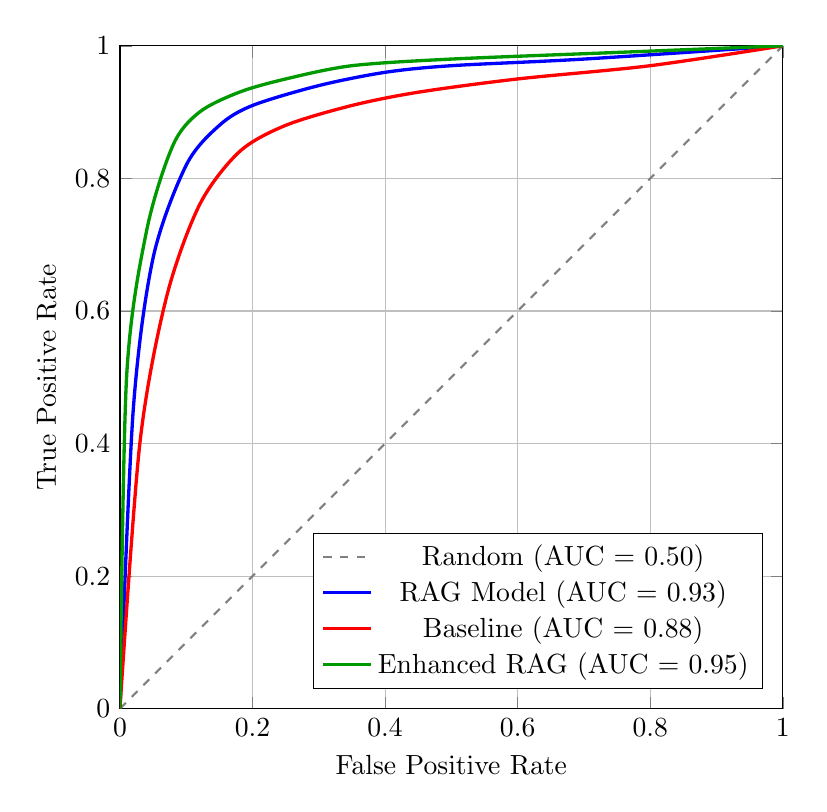
\begin{tikzpicture}
\begin{axis}[
    width=10cm,
    height=10cm,
    xlabel={False Positive Rate},
    ylabel={True Positive Rate},
    xmin=0, xmax=1,
    ymin=0, ymax=1,
    grid=major,
    legend pos=south east,
    axis equal
]

% Diagonal reference line (random classifier)
\addplot[dashed, gray, thick, domain=0:1] {x};
\addlegendentry{Random (AUC = 0.50)}

% ROC curve for Model 1
\addplot[blue, very thick, smooth] coordinates {
    (0.00, 0.00)
    (0.02, 0.45)
    (0.05, 0.68)
    (0.10, 0.82)
    (0.15, 0.88)
    (0.20, 0.91)
    (0.30, 0.94)
    (0.40, 0.96)
    (0.50, 0.97)
    (0.70, 0.98)
    (1.00, 1.00)
};
\addlegendentry{RAG Model (AUC = 0.93)}

% ROC curve for Model 2
\addplot[red, very thick, smooth] coordinates {
    (0.00, 0.00)
    (0.03, 0.40)
    (0.07, 0.62)
    (0.12, 0.76)
    (0.18, 0.84)
    (0.25, 0.88)
    (0.35, 0.91)
    (0.45, 0.93)
    (0.60, 0.95)
    (0.80, 0.97)
    (1.00, 1.00)
};
\addlegendentry{Baseline (AUC = 0.88)}

% ROC curve for Model 3
\addplot[green!60!black, very thick, smooth] coordinates {
    (0.00, 0.00)
    (0.01, 0.50)
    (0.04, 0.72)
    (0.08, 0.85)
    (0.12, 0.90)
    (0.18, 0.93)
    (0.25, 0.95)
    (0.35, 0.97)
    (0.50, 0.98)
    (0.75, 0.99)
    (1.00, 1.00)
};
\addlegendentry{Enhanced RAG (AUC = 0.95)}

\end{axis}
\end{tikzpicture}
